% !TeX root = main.tex

\hypertarget{concepts-of-hypothesis-testing}{%
\section{Concepts of Hypothesis
Testing}\label{concepts-of-hypothesis-testing}}

\hypertarget{the-basic-idea-of-hypothesis-testing}{%
\subsection{The Basic Idea of Hypothesis
Testing}\label{the-basic-idea-of-hypothesis-testing}}

\begin{itemize}
\item
  The testing procedure starts with an initial assumption that the
  statement on population parameter is true.
\item
  We test this initial assumption using a random sample. If the initial
  assumption is really the truth, then the test statistic from a random
  sample shouldn't be too far away from the center of the sampling
  distribution. Conversely, if the test statistic is too far
  away from the center, then we should not believe in the
  initial assumption.
\item
  To determine how far is too far away, we need to specify a threshold,
  a prior probability, or equivalently a critical value.
\item
  If the test statistic is at least extreme as the critical value, then
  the testing is significant enough to allow us to reject the initial
  assumption. Otherwise, we cannot draw a definite conclusion.
\item
  The prior probability measures the chance that the initial assumption
  was wrongly rejected.
\end{itemize}

\hypertarget{two-hypotheses}{%
\subsection{Two Hypotheses}\label{two-hypotheses}}

\begin{itemize}
\item
  A statistical \textbf{hypothesis} is a statement about a population
  parameter.
\item
  A \textbf{hypothesis test} is a process that uses sample statistics to
  test a \textbf{hypothesis}.
\item
  To test a population parameter, we choose a pair of hypotheses, the
  null hypothesis and the alternative hypothesis which are contradictory
  to each other.
\item
  The \textbf{null hypothesis}, denoted by \(H_0\), is the statement
  about the population parameter that is assumed to be true.
\item
  The \textbf{alternative hypothesis}, denoted \(H_a\), is a statement
  about the population parameter that is contradictory to the null
  hypothesis.
\end{itemize}

\begin{fullwidth}
  \colorbox{white}{
    \parbox{\linewidth}{\centering
      \textbf{Mathematical Symbols Used in \(H_0\) and \(H_a\)}
      
      \begin{longtable}[]{@{}cc@{}}
      \toprule()
      \(H_0\) & \(H_a\) \\
      \midrule()
      \endhead
      equal = & not equal \(\neq\) or greater than $>$ or less than
      $<$\\
      greater than or equal to \(\geq\) & less than $<$ \\
      less than or equal to $\leq$ & more than $>$ \\
      \bottomrule()
      \end{longtable}
    }}
\end{fullwidth}

\begin{example}

Identify the Null and the Alternative Hypotheses

\begin{enumerate}
\item
  Test a statement that the population mean is 1.
\item
  Test a statement that the population mean is more than 3.
\item
  Test a statement that the population mean is no more than 3.
\end{enumerate}

\end{example}


\hypertarget{the-logic-of-hypothesis-testing}{%
\subsection{The Logic of Hypothesis
Testing}\label{the-logic-of-hypothesis-testing}}

The logic of hypothesis testing and two types of error can be summarized in the following table.

\begin{fullwidth}
  \colorbox{white}{
\parbox{\linewidth}{\centering
  \begin{tabular}{l|*{2}{l}}
    ACTION & $H_0$  is Actually True & $H_0$  is Actually False\\
    \midrule
    Do not reject  $H_0$ & 	Correct Outcome	 & Type II error\\
    Reject  $H_0$ &	Type I Error & Correct Outcome
  \end{tabular}
}
  }
\end{fullwidth}


The interpretation of hypothesis testing is summarized in the following
table.

\begin{fullwidth}
  \colorbox{white}{
\parbox{\linewidth}{\centering
\begin{tabular}{l|p{0.35\linewidth}p{0.35\linewidth}}
  Action & If the claim to be tested is in \(H_0\) & If the claim to be tested is in \(H_a\) \\
  \midrule
  Reject \(H_0\) & There is enough evidence to reject the claim
  & There is enough evidence to support the claim \\
  Fail to Reject \(H_0\) & There is not enough evidence to reject the claim & There is not enough evidence to support the claim
\end{tabular}
}
  }
\end{fullwidth}

\hypertarget{type-of-errors-in-hypothesis-testing}{%
\subsection{Type of Errors in Hypothesis
Testing}\label{type-of-errors-in-hypothesis-testing}}

\begin{itemize}
\item
  Rejecting the null hypothesis when it is indeed true is called a
  \textbf{type I error}. The maximum allowable probability of making a
  type I error is called the \textbf{level of significance}, denoted by
  \(\alpha\). In other words,
  \[\alpha=P(\text{Type I error})= P(\text{reject a true }H_0).\]
\item
  Failing to reject the null hypothesis when the it is false is called a
  \textbf{type II error}. The probability of a type II error is usually
  denoted by \(\beta\). The \textbf{power of a hypothesis test}, equals
  \(1-\beta\), is the probability of rejecting the null hypothesis when
  it is false.
\end{itemize}

\begin{example}
Examples of Type I and Type II errors
\begin{center}
  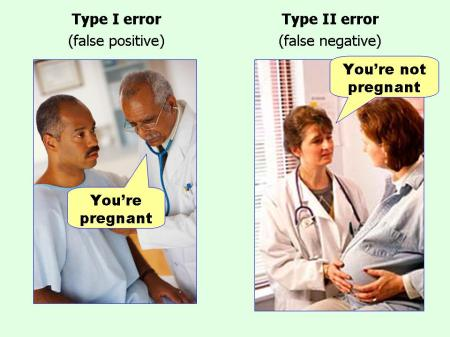
\includegraphics[width=0.9\textwidth]{Figures/type-i-and-type-ii-errors.jpg}\\
  \textbf{In the above picture, bubble texts are in \(H_a\)}
\end{center}
\end{example}
\vspace*{\baselineskip}

\hypertarget{type-of-tests}{%
\subsection{Type of Tests}\label{type-of-tests}}

\begin{itemize}
\item
  If \(H_a\) has the form \(\mu\neq \mu_0\) the test is called a
  \textbf{two-tailed test}.
\item
  If \(H_a\) has the form \(\mu<\mu_0\) the test is called a
  \textbf{left-tailed test}.
\item
  If \(H_a\) has the form \(\mu>\mu_0\) the test is called a
  \textbf{right-tailed test}.
\item
  Each of the last two forms is also called a \textbf{one-tailed test}.
\end{itemize}

\hypertarget{observed-significance}{%
\subsection{Observed Significance}\label{observed-significance}}

\begin{itemize}
\item
  To make a decision, one may also compare probabilities. The
  \textbf{observed significance} (\textbf{$P$-value}) of a test statistic is the probability of obtaining a sample statistic at least as extreme as the (observed) test statistic, given that the null hypothesis were true.
\item
  \(P\)-Value as Tail area

  \begin{longtable}[]{@{}lcc@{}}
  \toprule()
  Sign in \(H_a\) & \(\ne\) & \(<\) \\
  \midrule()
  \endhead
  \(P\)-value & Double of the tail area & Left tail area \\
  \bottomrule()
  \end{longtable}
\item
  Making decision by comparing the \(P\)-value with the significance
  level \(\alpha\):

  \begin{itemize}
  \item
    reject \(H_0\) if \(p\le \alpha\)
  \item
    fail to reject \(H_0\) if \(p>\alpha\).
  \end{itemize}
\end{itemize}

\begin{example}

Given the following testing hypotheses

\(H_{0}: p=0.50\) vs.~\(H_{a}: p\ne 0.50, n=360, \hat{p}=0.56\),

find the \(P\)-value for the test and make a decision at the 5\% level
of significance.

\end{example}
\vspace*{6\baselineskip}

\begin{example}

It is believed that a stock price for a particular company will grow at
a rate of \$5 per week with a standard deviation of \$1. An investor
believes the stock won't grow as quickly. The changes in stock price is
recorded for ten weeks and are as follows: \$4, \$3, \$2, \$3, \$1, \$7,
\$2, \$1, \$1, \$2. State the null and alternative hypotheses, find the
p-value, and identify the Type I and Type II errors.

\end{example}
\vspace*{6\baselineskip}

\hypertarget{practice}{%
\subsection{Practice}\label{practice}}

\begin{exercise}

Decide whether the following statements are true or false. Explain your reasoning.

\begin{itemize}
\item
  In case of a left-tailed test, we reject the null hypothesis if the
  sample statistic is significantly smaller than the hypothesized
  population parameter.
\item
  A \(P\)-value of 0.08 is more evidence against the null hypothesis
  than a \(P\)-value of 0.04.
\item
  The statement, ``the \(P\)-value is 0.03'', is equivalent to the
  statement, ``there is a 3\% probability that the null hypothesis is
  true''.
\item
  Even though you rejected the null hypothesis, it may still be true.
\item
  Failing to reject null hypothesis means the null hypothesis is true.
\item
  That the \(P\)-value of a sample statistic is \(p=0\) means the null
  hypothesis cannot be true.
\end{itemize}

\end{exercise}
\vspace*{4\baselineskip}

\begin{exercise}

Determine both Type I and Type II errors for the following scenario:

Assume a null hypothesis, \(H_0\), that states the percentage of adults
with jobs is at least 88\%. Identify the Type I and Type II errors from
these four statements.

\begin{enumerate}
\item
  Not to reject the null hypothesis that the percentage of adults who
  have jobs is at least 88\% when that percentage is actually less than
  88\%
\item
  Not to reject the null hypothesis that the percentage of adults who
  have jobs is at least 88\% when the percentage is actually at least
  88\%.
\item
  Reject the null hypothesis that the percentage of adults who have jobs
  is at least 88\% when the percentage is actually at least 88\%.
\item
  Reject the null hypothesis that the percentage of adults who have jobs
  is at least 88\% when that percentage is actually less than 88\%.
\end{enumerate}

\end{exercise}
\vspace*{2\baselineskip}

\begin{exercise}

  Determine if the following statements are true or false. Please explain your reasoning.

  \begin{itemize}
  \item
    The \(P\)-value of the test statistic is \(p = 0.06\). At the
    significance level \(\alpha=0.01\), the null hypothesis \(H_0\)
    should be rejected.
  \item
    A two-tailed test has larger probability of getting a type I error
    that a one-tailed test.
  \item
    That a test statistic falls in the rejection region means the
    \(P\)-value is smaller than the significance level.
  \end{itemize}

\end{exercise}
\vspace*{4\baselineskip}

\begin{exercise}

Suppose we're conducting a hypothesis testing for a population mean.
Find the \(P\)-value for each of the following testing scenario with the
given sample size \(n\) and the test statistics \(t\).

\begin{enumerate}
\item
  \(H_{0}: \mu=25 \text { vs. } H_{a} : \mu<25\), \(n=30\), \(t=-2.43\).
\item
  \(H_{0}: \mu=35 \text { vs. } H_{a} : \mu>35\), \(n=50\), \(t=2.13\).
\item
  \(H_{0}: \mu=-7.9 \text { vs. } H_{a} : \mu\ne-7.9\), \(n=40\),
  \(t=-1.99\).
\end{enumerate}

\end{exercise}

\begin{exercise}

It's a Boy Genetics Labs claim their procedures improve the chances of a
boy being born. The results for a test of a single population proportion
are as follows:

\begin{itemize}
\item
  \(H_0: p=0.50\), \(H_a:p>0.50\)
\item
  \(\alpha=0.01\)
\item
  \(p-\text{value}=0.025\)
\end{itemize}

Interpret the results and state a conclusion in simple, non-technical
terms.

\end{exercise}

\vspace*{6\baselineskip}

\hypertarget{lab-excel-functions-for-normal-distributions}{%
\subsection{Lab: Excel Functions for Normal
Distributions}\label{lab-excel-functions-for-normal-distributions}}

\begin{itemize}
\item
  Let \(Z\) be a standard normal random varaible. In Excel, \(P(Z<z)\)
  is given by \texttt{NORM.S.DIST(z,TRUE)}.
\item
  Let \(X\) be a normal random variable with mean \(\mu\) and standard
  deviation \(\sigma\), that is \(X\sim \mathcal{N}(\mu, \sigma^2)\). In
  Excel, \(P(X<x)\) is given by \texttt{NORM.DIST(x,mean,sd,TRUE)}.
\item
  When a cumulative probability \(p=P(X<x)\) of a normal random variable
  \(X\) is given, we can find \(x\) using\\ \texttt{NORM.INV(p,mean,sd)}.
\item
  When a cumulative probability \(p=P(Z<z)\) of a standard normal random
  variable \(Z\) is given, we can find \(z\) using
  \texttt{NORM.S.INV(p)}.
\end{itemize}

\hypertarget{lab-excel-functions-for-t-distributions}{%
\subsection{\texorpdfstring{Lab: Excel Functions for
\(T\)-Distributions}{Lab: Excel Functions for T-Distributions}}\label{lab-excel-functions-for-t-distributions}}

Suppose a Student's \(T\)-distribution has the degree of freedom
\(\text{df}=n-1\).

\begin{itemize}
\item
  To find a probability for a given \(T\)-value

  \begin{itemize}
  \item
    The area of the left tail of the \(T\)-value may be calculated by
    the function \texttt{T.DIST(t,df,true)}.
  \item
    The area of the right tail of the \(T\)-value may be calculated by
    the function \texttt{T.DIST.RT(t,\ df)}.
  \item
    The area of two tails of the \(T\)-value
    (\(t > 0\)) may be calculated by
    function \texttt{T.DIST.2T(t,df)}.
  \end{itemize}
\item
  To find the critical value for a given probability \(p\)

  \begin{itemize}
  \item
    When the area of the left tail is given, the function\\
    \texttt{T.INV(p,df)} may be used.
  \item
    When the area of both tails is given, the function\\
    \texttt{T.INV.2T(p,df)} may be used. This function is good for
    construction confidence interval.
  \end{itemize}
\end{itemize}

\begin{exercise}

Joon believes that 50\% of first-time brides in the United States are
younger than their grooms. She performs a hypothesis test to determine
if the percentage is the same or different from 50\%. Joon samples 100
first-time brides and 53 reply that they are younger than their grooms.
For the hypothesis test, find the \(p\)-value.

\end{exercise}
\vspace*{6\baselineskip}

\begin{exercise}

The average McDonald's restaurant generates \$3.7 million in sales each
year with a standard deviation of 0.7. Taylor wants to know if the
average sales generated by McDonald's restaurants in Missouri is greater
than the worldwide average. He surveys 24 restaurants in Missouri and
finds the following data (in millions of dollars):

\begin{tabular}{*{12}{c}}
  2.0 & 3.1 & 3.7 & 2.6 & 4.0 & 3.9 & 3.4 & 3.5 & 3.5 & 3.6 & 4.1 & 2.0 \\ 
  4.4 & 2.3 & 3.8 & 2.6 & 1.9 & 4.8 & 2.7 & 2.8 & 2.8 & 3.1 & 3.9 & 2.6  
\end{tabular}

Find the \(p\)-value.

\end{exercise}
\vspace*{6\baselineskip}

